% VUT FIT MITAI
% MSZ 2021/2022
% Author: Vladimir Dusek
% Login: xdusek27

%%%%%%%%%%%%%%%%%%%%%%%%%%%%%%%%%%%%%%%%%%%%%%%%%%%%%%%%%%%%%%%%%%%%%%%%%%%%%%%%

% Path to figures
\graphicspath{{tin/konecne_automaty/figures}}

%%%%%%%%%%%%%%%%%%%%%%%%%%%%%%%%%%%%%%%%%%%%%%%%%%%%%%%%%%%%%%%%%%%%%%%%%%%%%%%%

\chapter{TIN~--~Konečné automaty (jazyky přijímané KA, varianty KA, minimalizace KA, Mihill-Nerodova věta).}

%%%%%%%%%%%%%%%%%%%%%%%%%%%%%%%%%%%%%%%%%%%%%%%%%%%%%%%%%%%%%%%%%%%%%%%%%%%%%%%%

\section{Zdroje}

\begin{compactitem}
    \item \path{tin_2021_merged.pdf}
    \item \path{TIN_2020-09-22.mp4}
    \item \path{TIN_2020-09-29.mp4}
\end{compactitem}

%%%%%%%%%%%%%%%%%%%%%%%%%%%%%%%%%%%%%%%%%%%%%%%%%%%%%%%%%%%%%%%%%%%%%%%%%%%%%%%%

\section{Konečný automat}

\paragraph*{Konečný automat} Konečný automat (KA) je pětice $M = (Q, \Sigma, \delta, q_0, F)$, kde \begin{compactitem}
    \item $Q$ je konečná množina stavů;
    \item $\Sigma$ je vstupní abeceda;
    \item $\delta$ je přechodová funkce (parciální funkce), \begin{compactitem}
        \item $\delta : Q \times \Sigma \rightarrow 2^{Q}$;
    \end{compactitem}
    \item $q_0$ je výchozí stav, \begin{compactitem}
        \item $q_0 \in Q$;
    \end{compactitem}
    \item $F$ je množina koncových stavů, \begin{compactitem}
        \item $F \subseteq Q$;
    \end{compactitem}
\end{compactitem}

\paragraph*{Konfigurace} Konfigurace je dvojice $(q, w)$, kde \begin{compactitem}
    \item q je aktuální stav, $q \in Q$;
    \item w je nezpracovaná část vstupního řetězce, $w \in \Sigma^*$.
\end{compactitem}
Množina všech existujících konfigurací je pak $Q \times \Sigma^* $.

\paragraph*{Počáteční konfigurace} Počáteční konfigurace je taková konfigurace $(q, w)$, kde $q$ je výchozí stav.

\paragraph*{Finální konfigurace} Finální konfigurace je taková konfigurace $(q, w)$, kde $w = \epsilon$ je $q \in F$.

\paragraph*{Přechod} Přechod KA je binární relace (značíme $\vdash$) na množině konfigurací $\vdash ~ \subseteq (Q \times \Sigma^*) \times (Q \times \Sigma^*)$, taková, že $$ \forall q, q' \in Q ~ \forall w, w' \in \Sigma^* : (q, w) \vdash (q', w') \Rightarrow  \exists a \in \Sigma \land aw = w' \land w' \in \delta(w, a)$$

\paragraph*{Jazyk přijímaný KA} Mějme KA $M = (Q, \Sigma, \delta, q_0, F)$ a jazyk $L(M)$, který je přijímaný KA $M$. $$ L(M) = \{ w ~|~ w \in \Sigma^* \land (q_0, w) \vdash^* (q_f, \epsilon) \land q_f \in F \}$$

\paragraph*{Dosažitelné a nedosažitelné stavy} Mějme KA $M = (Q, \Sigma, \delta, q_0, F)$. Stav $q \in Q$ je dosažitelný, pokud platí $\exists w \in \Sigma^* : (q_0, w) \vdash^* (q, \epsilon)$. Stav je nedosažitelný, pokud není dosažitelný.

\paragraph*{Relace nerozlišitelnosti} Relace nerozlišitelnosti je binární relace nad množinou stavů. Stavy $p, q \in Q$ jsou rozlišitelné, jestliže existuje řetězec $w \in \Sigma^*$, pro který KA ze stavu $q$ skončí v nějakém $q_f \in F$, ale ze stavu $p$ nikoliv. Dva stavy jsou nerozlišitelné, pokud nejsou rozlišitelné. Formálně: nechť $p, q \in Q$ jsou rozlišitelné, pak platí $$ \forall w \in \Sigma^* : (p, w) \vdash^* (p', \epsilon) \land (q, w) \vdash^* (q', \epsilon) \land ( (p' \in F \land q' \not\in F) \lor (p' \not\in F \land q' \in F) ) $$

\paragraph*{k-nerozlišitelnost} \todo{todo}

%%%%%%%%%%%%%%%%%%%%%%%%%%%%%%%%%%%%%%%%%%%%%%%%%%%%%%%%%%%%%%%%%%%%%%%%%%%%%%%%

\section{Varianty konečného automatu}

Všechny varianty konečného automatu mají stejnou vyjadřovací sílu (jsou mezi sebou převoditelné).

\paragraph*{Nedeterministický konečný automat} Nedeterministický konečný automat (NKA) je výchozí konečný automat (NKA = KA).

\paragraph*{Deterministický konečný automat} Deterministický konečný automat (DKA) se od NKA liší pouze tvarem přechodové funkce. Formálně: \begin{compactitem}
    \item $\delta$ je přechodová funkce (parciální funkce), \begin{compactitem}
        \item $\delta : Q \times \Sigma \rightarrow Q$
    \end{compactitem}
\end{compactitem}

\paragraph*{Rozšířený konečný automat} Rozšířený konečný automat (RKA) se od NKA liší pouze tvarem přechodové funkce. Rozšiřuje ji o tzv. epsilon přechody. Formálně: \begin{compactitem}
    \item $\delta$ je přechodová funkce (parciální funkce), \begin{compactitem}
        \item $\delta : Q \times (\Sigma \cup \{ \epsilon \}) \rightarrow 2^Q$
    \end{compactitem}
\end{compactitem}

\paragraph*{Úplně definovaný konečný automat} Úplně definovaný konečný automat se od NKA liší pouze tvarem přechodové funkce. Formálně: \begin{compactitem}
    \item $\delta$ je přechodová funkce (totální funkce), \begin{compactitem}
        \item $\delta : Q \times \Sigma \rightarrow 2^Q$
        \item $\forall q \in Q ~ \forall a \in \Sigma : \delta(q, a) \in Q$
    \end{compactitem}
\end{compactitem}

\paragraph*{Redukovaný úplně definovaný deterministický konečný automat} Úplně definovaný DKA nazýváme redukovaný, jestliže žádný $q \in Q$ není nedosažitelný a žádná dvojice $p, q \in Q$ není nerozlišitelná.

\subsection{Převod NKA na DKA}

\begin{figure}[H]
    \centering
    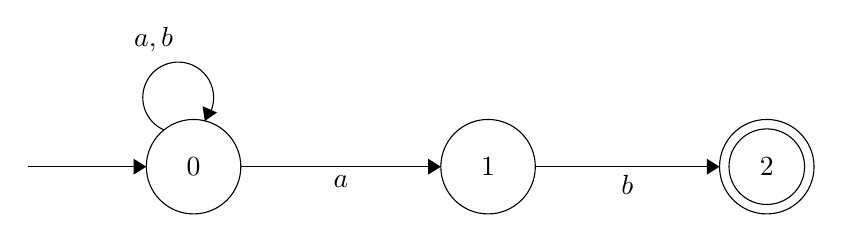
\begin{tikzpicture}[scale=0.2]
        \tikzstyle{every node}+=[inner sep=0pt]
        \draw [black] (18.2,-24.6) circle (3);
        \draw (18.2,-24.6) node {$0$};
        \draw [black] (36.9,-24.6) circle (3);
        \draw (36.9,-24.6) node {$1$};
        \draw [black] (54.6,-24.6) circle (3);
        \draw (54.6,-24.6) node {$2$};
        \draw [black] (54.6,-24.6) circle (2.4);
        \draw [black] (16.328,-22.271) arc (246.52881:-41.47119:2.25);
        \draw (15.66,-17.37) node [above] {$a,b$};
        \fill [black] (18.91,-21.7) -- (19.69,-21.16) -- (18.77,-20.76);
        \draw [black] (7.7,-24.6) -- (15.2,-24.6);
        \fill [black] (15.2,-24.6) -- (14.4,-24.1) -- (14.4,-25.1);
        \draw [black] (21.2,-24.6) -- (33.9,-24.6);
        \fill [black] (33.9,-24.6) -- (33.1,-24.1) -- (33.1,-25.1);
        \draw (27.55,-25.1) node [below] {$a$};
        \draw [black] (39.9,-24.6) -- (51.6,-24.6);
        \fill [black] (51.6,-24.6) -- (50.8,-24.1) -- (50.8,-25.1);
        \draw (45.75,-25.1) node [below] {$b$};
    \end{tikzpicture}
    \caption{Příklad NKA M.}
\end{figure}

\begin{figure}[H]
    \centering
    \includegraphics[width=0.75\linewidth]{nka_to_dka.pdf}
    \caption{Algoritmus převodu NKA na DKA.}
\end{figure}

\begin{figure}[H]
    \centering
    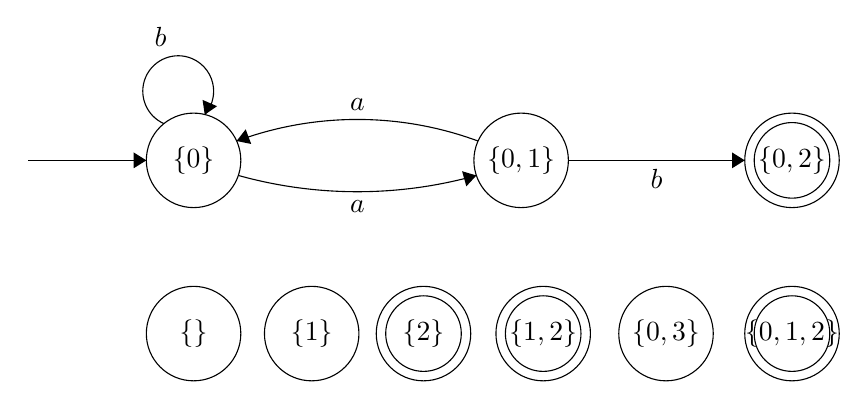
\begin{tikzpicture}[scale=0.2]
        \tikzstyle{every node}+=[inner sep=0pt]
        \draw [black] (17.5,-24.6) circle (3);
        \draw (17.5,-24.6) node {$\{0\}$};
        \draw [black] (38.3,-24.6) circle (3);
        \draw (38.3,-24.6) node {$\{0,1\}$};
        \draw [black] (55.5,-24.6) circle (3);
        \draw (55.5,-24.6) node {$\{0,2\}$};
        \draw [black] (55.5,-24.6) circle (2.4);
        \draw [black] (17.5,-35.6) circle (3);
        \draw (17.5,-35.6) node {$\{\}$};
        \draw [black] (25,-35.6) circle (3);
        \draw (25,-35.6) node {$\{1\}$};
        \draw [black] (39.7,-35.6) circle (3);
        \draw (39.7,-35.6) node {$\{1,2\}$};
        \draw [black] (39.7,-35.6) circle (2.4);
        \draw [black] (32.1,-35.6) circle (3);
        \draw (32.1,-35.6) node {$\{2\}$};
        \draw [black] (32.1,-35.6) circle (2.4);
        \draw [black] (55.5,-35.6) circle (3);
        \draw (55.5,-35.6) node {$\{0,1,2\}$};
        \draw [black] (55.5,-35.6) circle (2.4);
        \draw [black] (47.5,-35.6) circle (3);
        \draw (47.5,-35.6) node {$\{0,3\}$};
        \draw [black] (15.628,-22.271) arc (246.52881:-41.47119:2.25);
        \draw (15.4,-17.43) node [above] {$b$};
        \fill [black] (18.21,-21.7) -- (18.99,-21.16) -- (18.07,-20.76);
        \draw [black] (7,-24.6) -- (14.5,-24.6);
        \fill [black] (14.5,-24.6) -- (13.7,-24.1) -- (13.7,-25.1);
        \draw [black] (35.459,-25.558) arc (-74.4189:-105.5811:28.141);
        \fill [black] (35.46,-25.56) -- (34.55,-25.29) -- (34.82,-26.25);
        \draw (27.9,-27.09) node [below] {$a$};
        \draw [black] (41.3,-24.6) -- (52.5,-24.6);
        \fill [black] (52.5,-24.6) -- (51.7,-24.1) -- (51.7,-25.1);
        \draw (46.9,-25.1) node [below] {$b$};
        \draw [black] (20.235,-23.373) arc (110.28279:69.71721:22.112);
        \fill [black] (20.23,-23.37) -- (21.16,-23.56) -- (20.81,-22.63);
        \draw (27.9,-21.5) node [above] {$a$};
    \end{tikzpicture}
    \caption{DKA M.}
\end{figure}

\subsection{Převod RKA na DKA}

\todo{todo}

%%%%%%%%%%%%%%%%%%%%%%%%%%%%%%%%%%%%%%%%%%%%%%%%%%%%%%%%%%%%%%%%%%%%%%%%%%%%%%%%

\section{Minimalizace konečného automatu}

\begin{figure}[H]
    \centering
    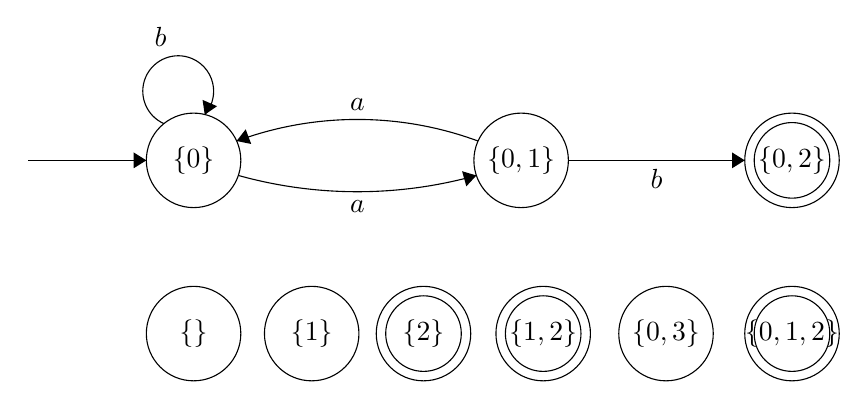
\begin{tikzpicture}[scale=0.2]
        \tikzstyle{every node}+=[inner sep=0pt]
        \draw [black] (17.5,-24.6) circle (3);
        \draw (17.5,-24.6) node {$\{0\}$};
        \draw [black] (38.3,-24.6) circle (3);
        \draw (38.3,-24.6) node {$\{0,1\}$};
        \draw [black] (55.5,-24.6) circle (3);
        \draw (55.5,-24.6) node {$\{0,2\}$};
        \draw [black] (55.5,-24.6) circle (2.4);
        \draw [black] (17.5,-35.6) circle (3);
        \draw (17.5,-35.6) node {$\{\}$};
        \draw [black] (25,-35.6) circle (3);
        \draw (25,-35.6) node {$\{1\}$};
        \draw [black] (39.7,-35.6) circle (3);
        \draw (39.7,-35.6) node {$\{1,2\}$};
        \draw [black] (39.7,-35.6) circle (2.4);
        \draw [black] (32.1,-35.6) circle (3);
        \draw (32.1,-35.6) node {$\{2\}$};
        \draw [black] (32.1,-35.6) circle (2.4);
        \draw [black] (55.5,-35.6) circle (3);
        \draw (55.5,-35.6) node {$\{0,1,2\}$};
        \draw [black] (55.5,-35.6) circle (2.4);
        \draw [black] (47.5,-35.6) circle (3);
        \draw (47.5,-35.6) node {$\{0,3\}$};
        \draw [black] (15.628,-22.271) arc (246.52881:-41.47119:2.25);
        \draw (15.4,-17.43) node [above] {$b$};
        \fill [black] (18.21,-21.7) -- (18.99,-21.16) -- (18.07,-20.76);
        \draw [black] (7,-24.6) -- (14.5,-24.6);
        \fill [black] (14.5,-24.6) -- (13.7,-24.1) -- (13.7,-25.1);
        \draw [black] (35.459,-25.558) arc (-74.4189:-105.5811:28.141);
        \fill [black] (35.46,-25.56) -- (34.55,-25.29) -- (34.82,-26.25);
        \draw (27.9,-27.09) node [below] {$a$};
        \draw [black] (41.3,-24.6) -- (52.5,-24.6);
        \fill [black] (52.5,-24.6) -- (51.7,-24.1) -- (51.7,-25.1);
        \draw (46.9,-25.1) node [below] {$b$};
        \draw [black] (20.235,-23.373) arc (110.28279:69.71721:22.112);
        \fill [black] (20.23,-23.37) -- (21.16,-23.56) -- (20.81,-22.63);
        \draw (27.9,-21.5) node [above] {$a$};
    \end{tikzpicture}
    \caption{DKA M.}
\end{figure}

\subsection{Eliminace nedosažitelných stavů}

\begin{figure}[H]
    \centering
    \includegraphics[width=0.9\linewidth]{eliminace_nedosazitelnych_stavu.pdf}
    \caption{Algoritmus eliminace nedosažitelných stavů.}
\end{figure}

\begin{figure}[H]
    \centering
    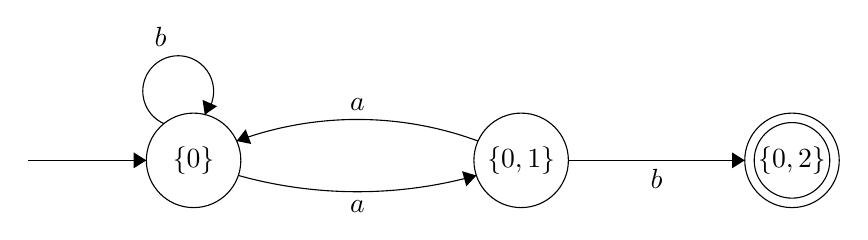
\begin{tikzpicture}[scale=0.2]
        \tikzstyle{every node}+=[inner sep=0pt]
        \draw [black] (18.5,-24.6) circle (3);
        \draw (18.5,-24.6) node {$\{0\}$};
        \draw [black] (39.3,-24.6) circle (3);
        \draw (39.3,-24.6) node {$\{0,1\}$};
        \draw [black] (56.5,-24.6) circle (3);
        \draw (56.5,-24.6) node {$\{0,2\}$};
        \draw [black] (56.5,-24.6) circle (2.4);
        \draw [black] (16.628,-22.271) arc (246.52881:-41.47119:2.25);
        \draw (16.4,-17.43) node [above] {$b$};
        \fill [black] (19.21,-21.7) -- (19.99,-21.16) -- (19.07,-20.76);
        \draw [black] (8,-24.6) -- (15.5,-24.6);
        \fill [black] (15.5,-24.6) -- (14.7,-24.1) -- (14.7,-25.1);
        \draw [black] (36.459,-25.558) arc (-74.4189:-105.5811:28.141);
        \fill [black] (36.46,-25.56) -- (35.55,-25.29) -- (35.82,-26.25);
        \draw (28.9,-27.09) node [below] {$a$};
        \draw [black] (42.3,-24.6) -- (53.5,-24.6);
        \fill [black] (53.5,-24.6) -- (52.7,-24.1) -- (52.7,-25.1);
        \draw (47.9,-25.1) node [below] {$b$};
        \draw [black] (21.235,-23.373) arc (110.28279:69.71721:22.112);
        \fill [black] (21.23,-23.37) -- (22.16,-23.56) -- (21.81,-22.63);
        \draw (28.9,-21.5) node [above] {$a$};
    \end{tikzpicture}
    \caption{DKA M bez nedosažitelných stavů.}
\end{figure}

\subsection{Převod DKA na úplně definovaný}

\begin{compactitem}
    \item Vstup: DKA $M = (Q, \Sigma, \delta, q_0, F)$
    \item Výstup: úplně definovaný DKA $M'$
    \item Metoda: \begin{compactenum}
        \item $\forall q \in Q ~ \forall a \in \Sigma : \delta(q, a) = \emptyset \Rightarrow \delta'(q, a) = q_s$
        \item $\forall a \in \Sigma : \delta'(q_s, a) = q_s$
        \item $M' = (Q \cup \{ q_s \}, \Sigma, \delta \cup \delta', q_o, F)$
    \end{compactenum}
    \item $q_s$ je tzv. \textit{sink} stav.
\end{compactitem}

\begin{figure}[H]
    \centering
    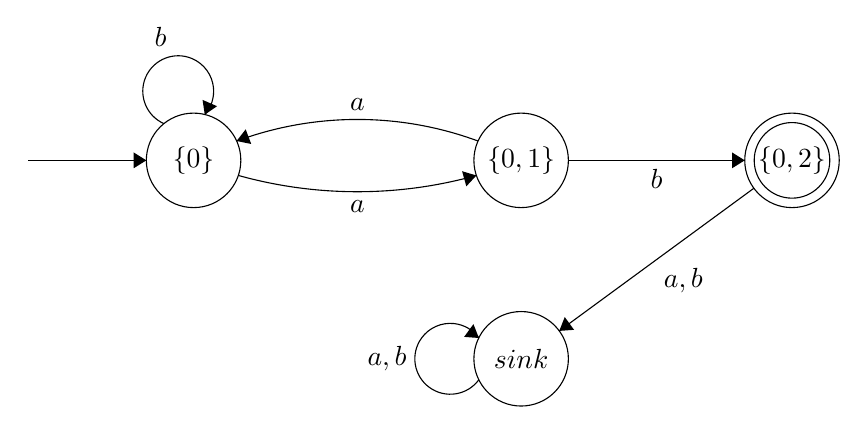
\begin{tikzpicture}[scale=0.2]
        \tikzstyle{every node}+=[inner sep=0pt]
        \draw [black] (18.4,-24.6) circle (3);
        \draw (18.4,-24.6) node {$\{0\}$};
        \draw [black] (39.2,-24.6) circle (3);
        \draw (39.2,-24.6) node {$\{0,1\}$};
        \draw [black] (56.4,-24.6) circle (3);
        \draw (56.4,-24.6) node {$\{0,2\}$};
        \draw [black] (56.4,-24.6) circle (2.4);
        \draw [black] (39.2,-37.2) circle (3);
        \draw (39.2,-37.2) node {$sink$};
        \draw [black] (16.528,-22.271) arc (246.52881:-41.47119:2.25);
        \draw (16.3,-17.43) node [above] {$b$};
        \fill [black] (19.11,-21.7) -- (19.89,-21.16) -- (18.97,-20.76);
        \draw [black] (7.9,-24.6) -- (15.4,-24.6);
        \fill [black] (15.4,-24.6) -- (14.6,-24.1) -- (14.6,-25.1);
        \draw [black] (36.359,-25.558) arc (-74.4189:-105.5811:28.141);
        \fill [black] (36.36,-25.56) -- (35.45,-25.29) -- (35.72,-26.25);
        \draw (28.8,-27.09) node [below] {$a$};
        \draw [black] (42.2,-24.6) -- (53.4,-24.6);
        \fill [black] (53.4,-24.6) -- (52.6,-24.1) -- (52.6,-25.1);
        \draw (47.8,-25.1) node [below] {$b$};
        \draw [black] (21.135,-23.373) arc (110.28279:69.71721:22.112);
        \fill [black] (21.13,-23.37) -- (22.06,-23.56) -- (21.71,-22.63);
        \draw (28.8,-21.5) node [above] {$a$};
        \draw [black] (53.98,-26.37) -- (41.62,-35.43);
        \fill [black] (41.62,-35.43) -- (42.56,-35.36) -- (41.97,-34.55);
        \draw (49.5,-31.4) node [below] {$a,b$};
        \draw [black] (36.52,-38.523) arc (-36:-324:2.25);
        \draw (31.95,-37.2) node [left] {$a,b$};
        \fill [black] (36.52,-35.88) -- (36.17,-35) -- (35.58,-35.81);
    \end{tikzpicture}
    \caption{Úplně definovaný DKA M.}
\end{figure}

\subsection{Převod úplně definovaného DKA na redukovaný}

\begin{figure}[H]
    \centering
    \includegraphics[width=0.9\linewidth]{prevod_na_redukovany_dka.pdf}
    \caption{Algoritmus převodu úplně definovaného DKA na redukovaný.}
\end{figure}

\subsection{Odstranění \textit{sink} stavu}

\begin{compactitem}
    \item Vstup: DKA $M = (Q, \Sigma, \delta, q_0, F)$
    \item Výstup: DKA $M'$ bez \textit{sink} stavu
    \item Metoda: \begin{compactenum}
        \item $Q' = \{ q ~|~ q \in Q \land w \in \Sigma^* \land q_f \in F \land (q, w) \vdash^* (q_f, \epsilon) \}$
        \item $\delta' = \{ (p, a, q) ~|~ \delta(p, a) = q \land q \not\in Q - Q' \}$
        \item $M' = \{ Q', \Sigma, \delta', q_0, F \}$
    \end{compactenum}
\end{compactitem}

\begin{figure}[H]
    \centering
    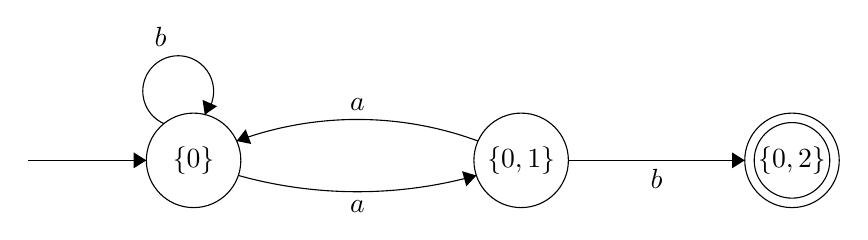
\begin{tikzpicture}[scale=0.2]
        \tikzstyle{every node}+=[inner sep=0pt]
        \draw [black] (18.5,-24.6) circle (3);
        \draw (18.5,-24.6) node {$\{0\}$};
        \draw [black] (39.3,-24.6) circle (3);
        \draw (39.3,-24.6) node {$\{0,1\}$};
        \draw [black] (56.5,-24.6) circle (3);
        \draw (56.5,-24.6) node {$\{0,2\}$};
        \draw [black] (56.5,-24.6) circle (2.4);
        \draw [black] (16.628,-22.271) arc (246.52881:-41.47119:2.25);
        \draw (16.4,-17.43) node [above] {$b$};
        \fill [black] (19.21,-21.7) -- (19.99,-21.16) -- (19.07,-20.76);
        \draw [black] (8,-24.6) -- (15.5,-24.6);
        \fill [black] (15.5,-24.6) -- (14.7,-24.1) -- (14.7,-25.1);
        \draw [black] (36.459,-25.558) arc (-74.4189:-105.5811:28.141);
        \fill [black] (36.46,-25.56) -- (35.55,-25.29) -- (35.82,-26.25);
        \draw (28.9,-27.09) node [below] {$a$};
        \draw [black] (42.3,-24.6) -- (53.5,-24.6);
        \fill [black] (53.5,-24.6) -- (52.7,-24.1) -- (52.7,-25.1);
        \draw (47.9,-25.1) node [below] {$b$};
        \draw [black] (21.235,-23.373) arc (110.28279:69.71721:22.112);
        \fill [black] (21.23,-23.37) -- (22.16,-23.56) -- (21.81,-22.63);
        \draw (28.9,-21.5) node [above] {$a$};
    \end{tikzpicture}
    \caption{DKA M bez \textit{sink} stavu.}
\end{figure}

%%%%%%%%%%%%%%%%%%%%%%%%%%%%%%%%%%%%%%%%%%%%%%%%%%%%%%%%%%%%%%%%%%%%%%%%%%%%%%%%

\section{Mihill-Nerodova věta}

\todo{todo}
